\documentclass[11pt,a4paper]{article}
\usepackage[utf8]{inputenc}
\usepackage[spanish]{babel}	%Idioma
\usepackage{amsmath}
\usepackage{amsfonts}
\usepackage{amssymb}
\usepackage{graphicx} %Añadir imágenes
\usepackage{geometry}	%Ajustar márgenes
\usepackage[export]{adjustbox}[2011/08/13]
\usepackage{float}
\restylefloat{table}
\usepackage{hyperref}
\usepackage{titling}
\usepackage{minted}
%Opciones de encabezado y pie de página:
\usepackage{fancyhdr}
\pagestyle{fancy}
\lhead{}
%\rhead{}
\lfoot{Técnicas de los Sistemas Inteligentes}
\cfoot{}
\rfoot{\thepage}
\renewcommand{\headrulewidth}{0.4pt}
\renewcommand{\footrulewidth}{0.4pt}
%Opciones de fuente:
\renewcommand{\familydefault}{\sfdefault}
\setlength{\parindent}{0pt}
\setlength{\headheight}{15pt}
\setlength{\voffset}{10mm}

% Custom colors
\usepackage{color}
\definecolor{deepblue}{rgb}{0,0,0.5}
\definecolor{deepred}{rgb}{0.6,0,0}
\definecolor{deepgreen}{rgb}{0,0.5,0}

\usepackage{listings}

\pretitle{%
  \centering
  \LARGE
  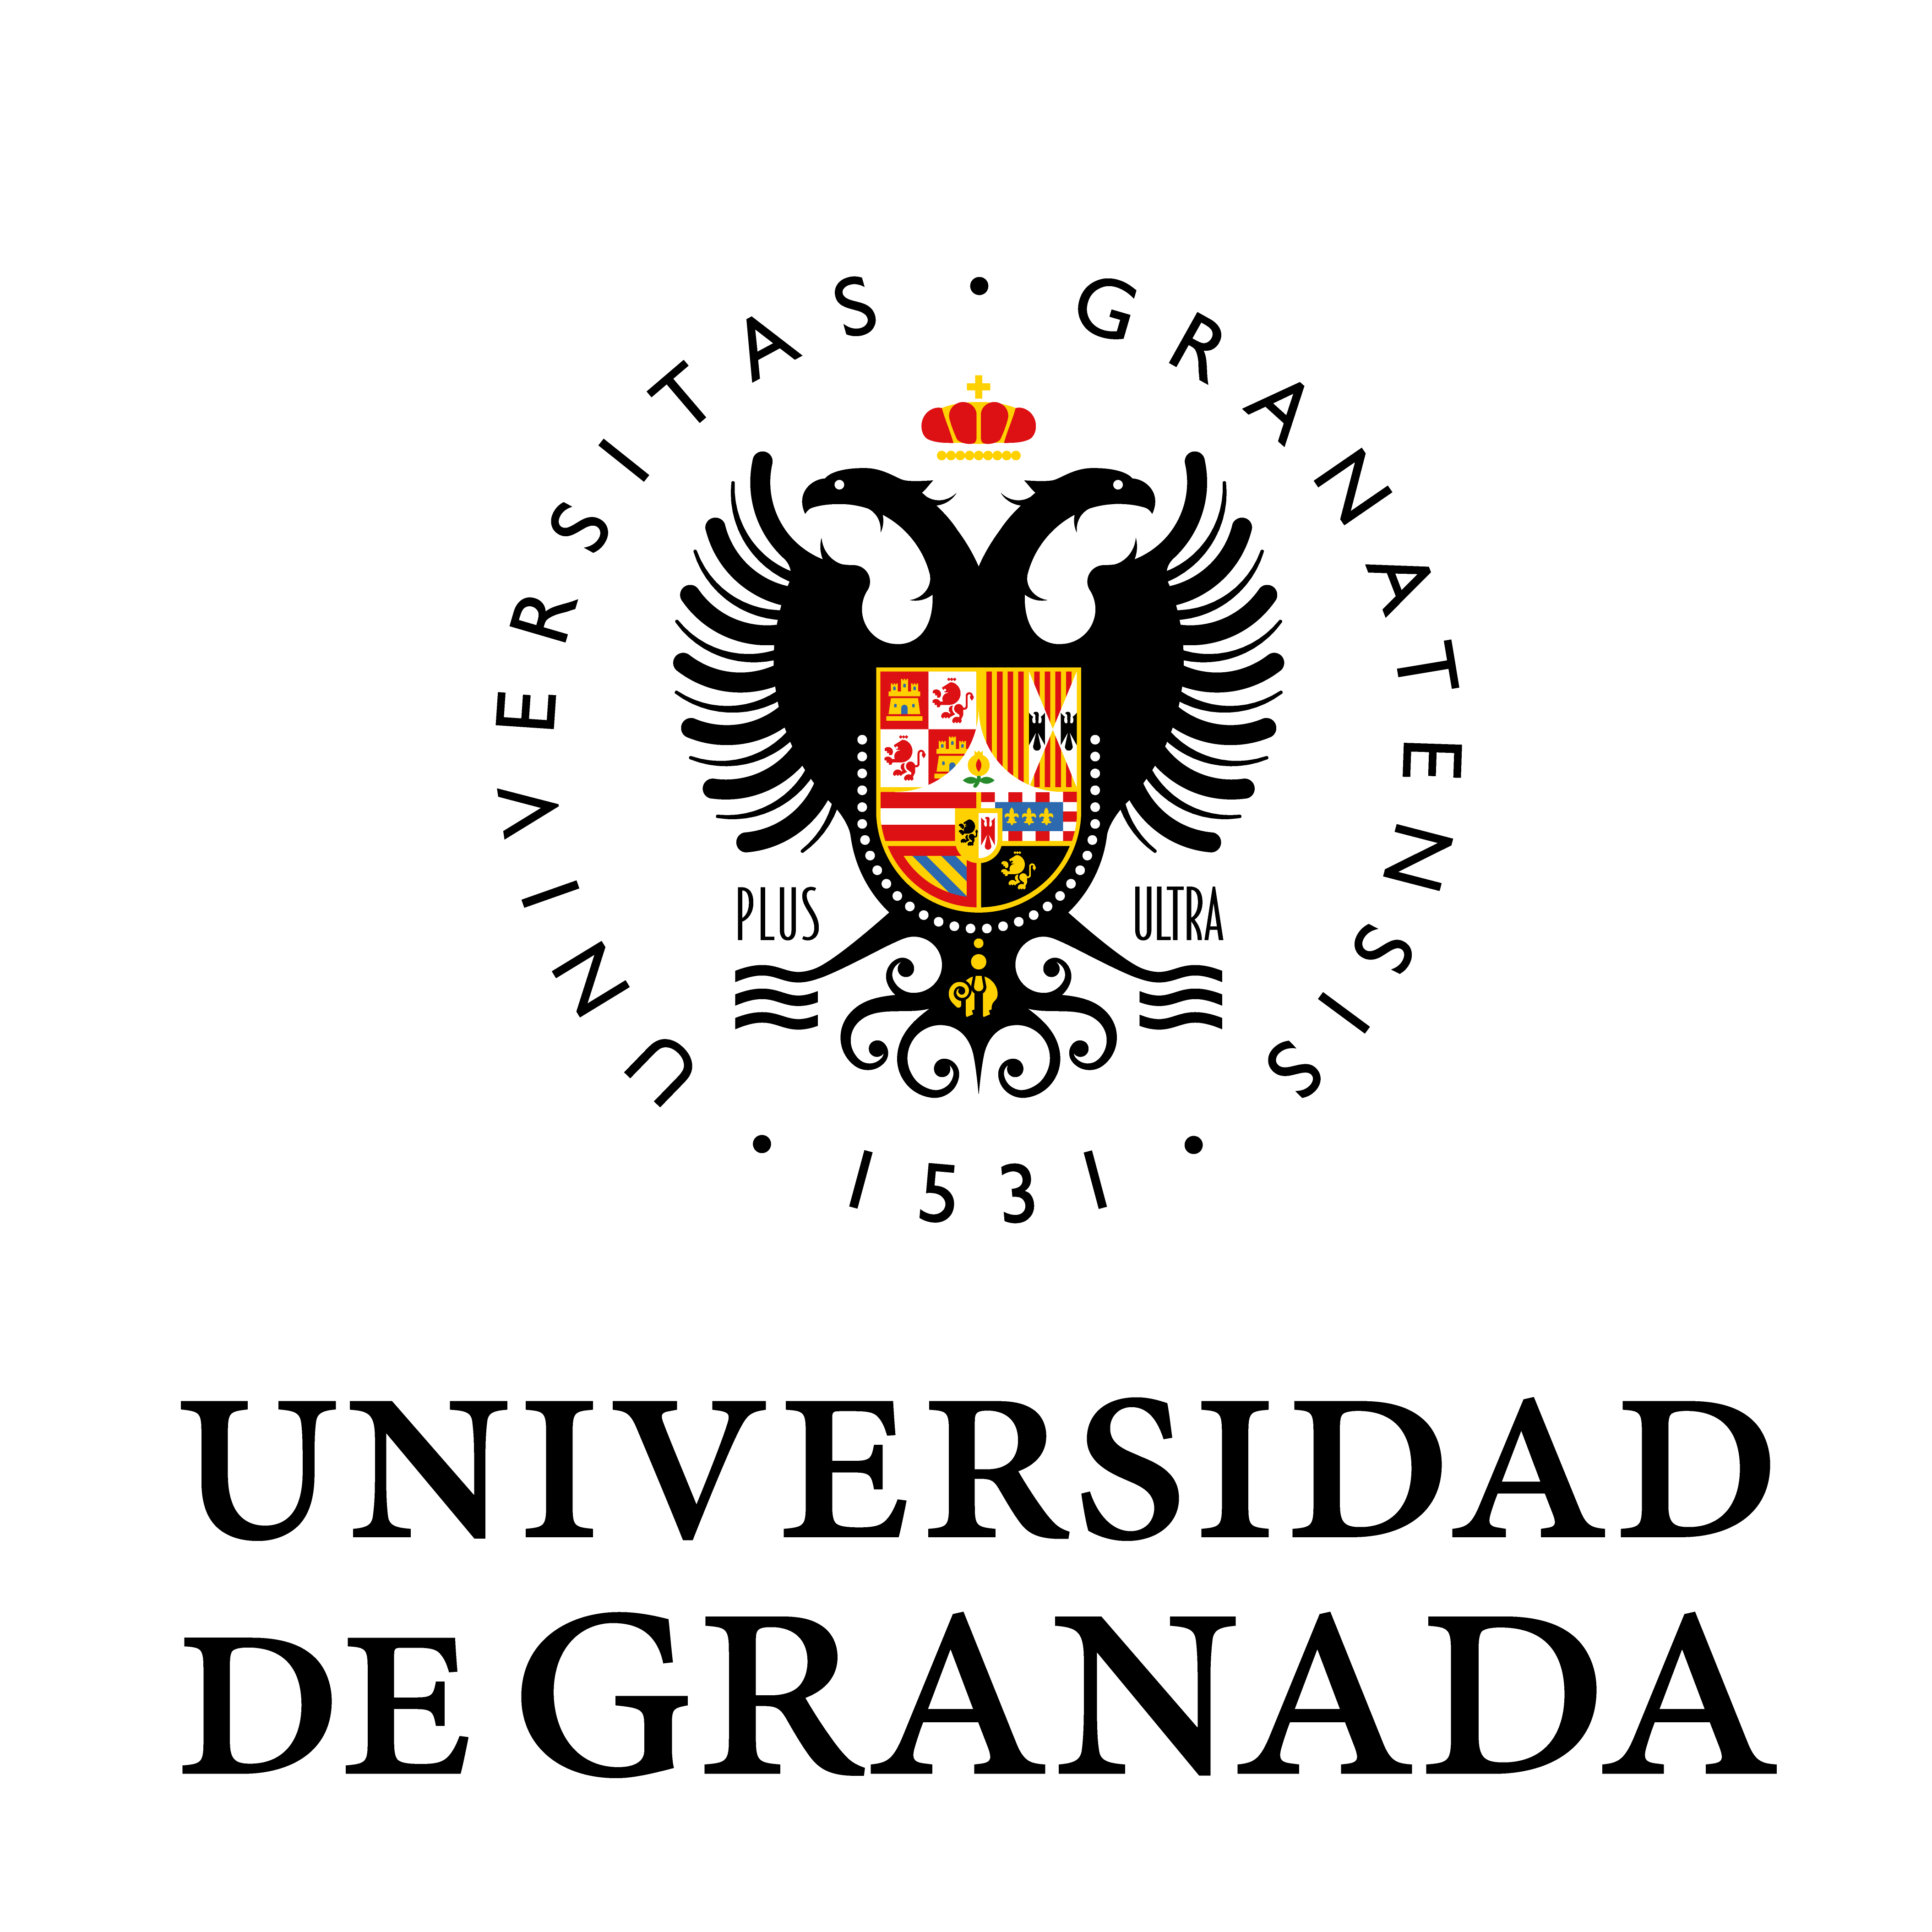
\includegraphics[scale=0.5]{logo.png}\\[\bigskipamount]
}
\posttitle{\begin{center} \end{center}}

\author{	Juan Ocaña Valenzuela}
\title{\textbf{Práctica 1: boulder dash}}

\begin{document}

\thispagestyle{empty}

\maketitle

\newpage

\tableofcontents

\newpage

\section{Descripción general de la solución}

\textbf{Nota:} originalmente el Agente iba a presentar un comportamiento mucho más complejo del que aparece
en la entrega, pero debido a una mala planificación del tiempo me he visto obligado a simplificar su 
funcionamiento. En este punto detallaré tanto los comportamientos que realiza como las ideas que, pese a no estar implementadas,
creo que funcionarían bien y pensaba programar.

\subsection{Comportamiento actual}
Nuestro agente presenta un comportamiento deliberativo a la hora de encontrar la ruta a seguir para conseguir las gemas y 
dirigirse a la puerta, y reactivo para huir de los enemigos que deambulan por el mapa.

\subsubsection{Clase GameState}
Como la mayoría de datos con los que trabajará serán las posiciones de los elementos extraídos de las observaciones, se ha 
encapsulado el estado del juego en la clase GameState, con métodos que devolverán información útil sobre el estado del juego en
un momento dado. 

\textbf{Atributos:}
\begin{itemize}
\item   private StateObservation obs;
\item   private PlayerObservation player;
\item   private Agent pat;
\item   private ArrayList<Observation>[][] map;
\end{itemize}

Guardamos el estado actual del juego en \textit{obs}, y el estado del jugador en \textit{player}, así como una referencia al 
agente en \textit{pat} y el mapa, que obtenemos con getObservationGrid().

La mayoría de los métodos utilizados devolverán puntos del mapa, representados con objetos de la clase tools.Vector2d.


\subsubsection{Pathfinder}
Se ha utilizado la clase PathFinder.java incluida en GVGAI, con ligeras modificaciones para calcular con un 
algoritmo A* la ruta entre dos puntos (representados como Vector2d, como se ha mencionado anteriormente). 

La ventaja que ofrece esta clase es la posibilidad de pasarle como argumentos al constructor el ID de los objetos que queremos 
evitar a la hora de encontrar una ruta. En la práctica utilizaremos dos objetos de esta clase: \textit{pf}, destinado a calcular la 
ruta que debe seguir nuestro agente; y \textit{bugFinder}, que comprobará si existe una ruta de tierra excavada entre un enemigo y nuestro agente, para así saber si supone una amenaza o no.


\subsubsection{Coger gemas e ir al portal}
Nuestro agente trabajará de la siguiente forma: obtendrá una lista de las gemas disponibles en el mapa y calculará la distancia de manhattan con cada una de ellas, seleccionando la más cercana como su objetivo. Calculará una ruta entre su posición y la de la gema con el objeto \textit{pf}, obteniendo una lista de posiciones a recorrer, y lo hará como sigue:

\begin{itemize}
\item Si está en la misma orientación que la próxima posición del mapa, avanza en esa dirección y pasa a considerar la siguiente
posición del plan.
\item Si no está orientado hacia la próxima posición, gira hacia ella y sigue considerando la misma posición del plan para la siguiente acción.
\item Una vez conseguidas las gemas necesarias, calculará la ruta hacia la salida y se dirigirá a ella.
\end{itemize}


\subsubsection{Esquivar bichos}
El comportamiento reactivo para esquivar bichos consiste en lo siguiente:
Se establece un área de peligro de radio 2, es decir, todas las casillas que estén a distancia 2 o menos del agente
se considerarán para comprobar si estamos en peligro de muerte por bicho.

El agente obtendrá una lista de todos los enemigos del mapa, y calculará la distancia de manhattan con cada uno de ellos.
Si alguno está a distancia 2 o menos, se activará el <<modo peligro>>, que consistirá en huir a la dirección contraria a la que se encuentra.

Este comportamiento presenta fallas, y es muy mejorable.

\subsubsection{Buffer de movimientos}
Para realizar acciones que requieran dos movimientos en lugar de uno, el agente utiliza una variable, \textit{actionBuffer}, que permanecerá con el valor \textit{Types.ACTIONS.ACTION\_NIL} hasta que se le asigne otro valor. Al principio del método \textit{act} se comprobará si este valor es distinto de NIL, y si lo es, ejecutará dicha acción y vaciará el buffer, sin tener en cuenta nada más en ese turno.



\subsection{Ideas sobre posibles mejoras}
Una de las ideas que se me pasó por la cabeza fue utilizar un mapa de pesos para calcular las rutas entre el agente, las gemas y el portal evitando y esquivando a los enemigos y las acciones de potencial peligro. Para ello, cada bicho tendría un área alrededor de un radio determinado, y las casillas irían aumentando de peso gradualmente a medida que fuesen más próximas al mismo. Para situaciones en las que al coger una gema o pasar por rocas podríamos morir sepultados, se tendría en cuenta ese caso especial y la acción de pasar por debajo de una roca sería más costosa que rodear dicha posición. Así, si no quedase más remedio pasaría por ahí, pero por norma general no lo haría, salvo que compensase.

Otra idea, compartida con unos compañeros, fue la de comprobar si un bicho estaba encerrado o no, y evitar en la medida de lo posible liberarlo, estableciendo los límites de la zona de tierra excavada con un coste alto, para reducir considerablemente las situaciones de riesgo.

Por último, a la hora de huir de uno o varios enemigos, se elaboraría un mapa de peligro en el que se aumentaría gradualmente el coste de las acciones que nos acercasen a él de forma considerable. Si hubiese más de un bicho en la zona de peligro, esto nos llevaría a hir de todos ellos, si fuese posible.


\section{Conclusiones}
Se ha hecho lo que se ha podido en el poco tiempo que me he dejado para hacer la práctica. Comprendo la baja complejidad y los pobres resultados del Agente, y no es mi intención justificarlo. De cara a las siguientes prácticas intentaré planificar mejor mi tiempo y estar a la altura. Me da pena tener tantas ideas interesantes para esta práctica y no haber podido llevarlas a cabo, pero me lo he buscado.

\end{document}